\documentclass[a4paper]{article}

\usepackage[english]{babel}
\usepackage[utf8]{inputenc}
\usepackage{amsmath}
\usepackage{graphicx}
\usepackage[colorinlistoftodos]{todonotes}
\usepackage{url}
\usepackage[margin=1in]{geometry} 
\usepackage{verbatim}

% using the todonotes package in some nice ways (see packages.tex)
\newcommand{\add}[2][]{\todo[color=blue!40,#1]{#2}{}}
\newcommand\optional[2][]{\todo[inline, color=cyan!40, caption={2do},
	#1]{\begin{minipage}{\textwidth-4pt}#2\end{minipage}}{}}

% math macros
\newcommand{\set}[1]{\boldsymbol{#1}}
\renewcommand{\vec}[1]{\mathbf{#1}}

% % commands for easy referencing
\newcommand{\fref}[1]{Figure~\ref{#1}}
\newcommand{\tref}[1]{Table~\ref{#1}}
\newcommand{\eref}[1]{Equation~\ref{#1}}
\newcommand{\cref}[1]{Chapter~\ref{#1}}
\newcommand{\sref}[1]{Section~\ref{#1}}
\newcommand{\aref}[1]{Appendix~\ref{#1}}

% fancy source code listings: http://stackoverflow.com/questions/741985/latex-source-code-listing-like-in-professional-books
% usage: \lstinputlisting[label=samplecode,caption=A sample]{sourceCode/HelloWorld.java}
\definecolor{light-gray}{gray}{0.95}
\usepackage{listings}
\usepackage{courier}
\lstset{
         basicstyle=\footnotesize\ttfamily, % Standardschrift
         numbers=left,               % Ort der Zeilennummern
         numberstyle=\tiny,          % Stil der Zeilennummern
         stepnumber=0,               % Abstand zwischen den Zeilennummern
         numbersep=5pt,              % Abstand der Nummern zum Text
         tabsize=2,                  % Groesse von Tabs
         extendedchars=true,         %
         breaklines=true,            % Zeilen werden Umgebrochen
         keywordstyle=\color{red},
         stringstyle=\color{white}\ttfamily, % Farbe der String
         showspaces=false,           % Leerzeichen anzeigen ?
         showtabs=false,             % Tabs anzeigen ?
         xleftmargin=0pt,
         framexleftmargin=10pt,
         framexrightmargin=10pt,
         framexbottommargin=0pt,
         backgroundcolor=\color{light-gray},
         showstringspaces=false      % Leerzeichen in Strings anzeigen ?
}

\lstdefinestyle{customc}{
  	belowcaptionskip=1\baselineskip,
  	breaklines=true,
  	%frame=L,
  	language=BASH,
  	showstringspaces=false,
 	basicstyle=\footnotesize\ttfamily\color{blue!40!black},
 	keywordstyle=\bfseries\color{green!40!black},
  	commentstyle=\itshape\color{purple!40!black},
  	%identifierstyle=\color{blue}, %color of actual code
 	stringstyle=\color{orange},
    numbers=left,               % Ort der Zeilennummern
    numberstyle=\tiny,          % Stil der Zeilennummern
    stepnumber=2,               % Abstand zwischen den Zeilennummern
    numbersep=5pt,              % Abstand der Nummern zum Text
    tabsize=2,                  % Groesse von Tabs
    extendedchars=true,         %
    showspaces=false,           % Leerzeichen anzeigen ?
    showtabs=false,             % Tabs anzeigen ?
  	xleftmargin=\parindent,
    framexleftmargin=10pt,
    framexrightmargin=10pt,
    framexbottommargin=0pt,
    backgroundcolor=\color{light-gray},
}

\lstset{style=customc}% i have deleted "escapechar=@,"


\title{Robocup Tutorial}

\author{Mohsen Kaboli, Maximilian Diehl}

\date{\today}

\begin{document}
\maketitle

\section{Building the working environment}

\subsection{System}
The working environment is \textbf{Ubuntu 14.04}, which is already installed on all the computers and laptops in the lab. If it's your first time to work with it, please get in contact with the supervisors and we will provide some useful tutorials for help.

\subsection{Prerequisite for building the project}
To build the project, some software are required. More details are discussed in \cite{BHuman2015}(cf. 2.3.4).\\
To sum up, it could be done with following commands:
\begin{lstlisting}
sudo apt-get install qt4-dev-tools libglew-dev libxm12-dev clang graphviz
\end{lstlisting}
If there is any problem, you can install the package one by one to check where the problem is exactly.
\subsection{Downloading the package}
\begin{itemize}
\item Go to the Github repository of B-Human team and download the required packages. 
Please take care that we use \textbf{coderelease2015}. 
\item Download 32 bit version of \textsl{Naoqi} (\textsl{C++ SDK 2.1.4 Linux 32}), which can be found in Gitlab repository/SoftwareTools.
\item Installed with the command:
\begin{lstlisting}
cd <BHuman-CodeRelease>/Install
./installAlcommon <pathto32bitC++NAOQi.tar.gz>
\end{lstlisting}
\end{itemize}


\subsection{Building the project}
\label{sec: building the project}
The whole project can be built with:
\begin{lstlisting}
cd <BHuman-CodeRelease>/Make/Linux
make all
\end{lstlisting}
Also, different components can be built seperately, which are:
\begin{itemize}
\item bush
\item Controller
\item libbhuman
\item libgamectrl
\item libqxt
\item Nao
\item qtpropertybrowser
\item SimRobot
\item SimRobotCore2
\item SimRobotEditor
\item SimRobotHelp
\item SimulatedNao
\end{itemize}
All components canbe built in three configurations, \textit{Release, Develop} and \textit{Debug}. The default seting is \textit{Develop} like:
\begin{lstlisting}
cd <BHuman-CodeRelease>/Make/Linux
make <component> [CONFIG=<configuration>]
\end{lstlisting}
For more details about the description of these components  see \cite{BHuman2015}(cf. 2.2)
\clearpage


\begin{comment}


\section{(Option) Flashing the Robot}
This part is provided for a  new robot. Although all robots have already been flashed, it is meaningful to do everything from scratch again to understand the whole procedure.

\subsection{Preparing the USB and flashing}
All the tools and image file that we need are in the Gitlab repository/Softwares.\\
And please prepare an empty USB disk which will be written the atom system image file.\\ 
The atom system image and corresponding \textit{Flasher} should be downloaded from \url{https://community.aldebaran.com}. Then the following steps should be done:
\begin{itemize}
    \item Extract the \textit{Flasher} and execute
    \begin{lstlisting}
cd <Flasher>
sudo ./flasher
    \end{lstlisting}
    \item \textit{Factor reset} should be chosen before flashing.
    \item Click the ``write" button and wait for 2 minutes it will finish the writing.
    \item Make sure the NAO is turned off before you plug in the USB disk.
    \item Plug the USB to the backside of NAO and press the chest button until the chest turns blue(around 5 seconds).
    \item The installation process will start and be monitored by the LED lights around NAO's ears. It takes around 10 minutes. 
    \item When finished, the chest button should be pressed and NAO will tell its initial IP-Address. Note down the IP-Address for future  use. If it doesn't speak the IP address just wait for one minute and press the chest button again. It always takes time to initialize the system. It may rotate the head randomly and seems to track your face, so you can remove the USB disk to prevent breaking down your USB disk.
\end{itemize}
More details for the flashing procedure can be found at \url{http://doc.aldebaran.com/2-1/nao/boot_process_nao.html#upgrading-process-nao}.

\subsection{Create the robot}
Before creating the robot, configure  $AAA.BBB$ in template file \emph{wired}(Line 6) in \emph{Install/Network}.\\
Each robot has its unique IP-Address, which looks like $AAA.BBB.CCC.DDD$ (IPv4 IP-Address). Here, we set $AAA = 169, BBB=254$ for all robots' wired configuration (For wireless settings, we set $AAA=10, BBB=0$). And $CCC$ is for the team ID and $DDD$ for robot ID. For example, $169.254.29.173$ is the robot $173$ from team $29$.  In addition, we should also assign a nickname to it such as \emph{Neue}.

Then the new robot can be created like:
\begin{lstlisting}
cd <BHuman-CodeRelease>/Install
./createRobot -t CCC -r DDD <nickname> # CCC.DDD should be the IP address on the robot leg, the target IP address.
./addRobotIds -ip <Initial IP-Address> <nickname> # The initial IP address which NAO speaks out
\end{lstlisting}
This step is very important, it will create the file robot.cfg.
\subsection{Conguration of the Network}
The robot can only be connected with cables after reflashing. 
\begin{itemize}
\item Connect the robot with the computer and add a \emph{Ethernet Connection}. 
\item Set the \emph{method} in \emph{IPv4 Settings} as \emph{link-local only}. 
\item Now the computer could connect with the robot. Try 
\begin{lstlisting}
ssh nao@<Initial IP-Address>
\end{lstlisting}
to check the reachablity of the robot. The IP-Address is the one given by Nao after flashing.
If it doesn't work add sudo before the command.
\end{itemize}


\subsection{Copy the compiled code to robots}
After connecting to the robot successfully, we can install the robot and copy the complied code to it.\\ 
To do this, it can be done with
\begin{lstlisting}
cd <BHuman-CodeRelease>/Install
./installRobot <initial IP-Address> # Pay attention! Initial IP address!!
\end{lstlisting}
Follow the instruction in the terminal, e.g. just enter the password ``root" when it requires.
After this step, the robot IP-Address will be changed into $AAA.BBB.CCC.DDD$. (The one you assigned)\\
Reconnet the robot with \emph{ssh} and copy the compiled code to robot with:
\begin{lstlisting}
cd <BHuman-CodeRelease>/Make/Linux
./copyfiles Develop AAA.BBB.CCC.DDD -r
\end{lstlisting}
More options for the command $copyfiles$ can be found in \cite{BHuman2015}(cf. 2.5)
\subsection{Setting up the wireless configuration}
To set up the wireless configuration, the files in \emph{Install/Network/Profiles} should be configured. Create  a new \emph{NAOwifi.wpa} file, the syntax can be referred from the \emph{example.wpa} file. One example looks like
\begin{lstlisting}
ctrl_interface=/var/run/wpa_supplicant
ctrl_interface_group=0
ap_scan=1

network={
  ssid="NAOSWIFI"
  key_mgmt=WPA-PSK
  pairwise=TKIP # Pay attention! Here should be modified as TKIP
  group=TKIP
  psk="naoapp99"
}

\end{lstlisting}
Then the wireless profiles can be updated with 
\begin{lstlisting}
cd <BHuman-CodeRelease>/Make/Linux
./copyfiles Develop AAA.BBB.CCC.DDD -w NAOwifi.wpa
\end{lstlisting}
Plug out the cable and connect to the WIFI (\emph{NAOSWIFI}) with the password \emph{naoapp99}. Now you should be able to connect with the robot through \emph{ssh} command.
\clearpage
\end{comment}



\section{Connecting to Nao and playing around in SimRobot}
\subsection{Connecting to Nao}
After previous setting-up steps, Nao can be connected with both cable and WIFI. The reachability can be checked with $ssh$ command in the terminal. After successful connection, some commands can be executed directly in the terminal to control the robot. 
\begin{itemize}
	\item \textbf{nao start\textbar stop\textbar restart} starts, stops or restarts NAOqi.
	\item \textbf{bhumand start\textbar stop\textbar restart} starts, stops or restarts the bhuman executable.
	\item \textbf{status} shows the status of NAOqi and bhuman.
	\item \textbf{stop} stops running instances of NAOqi and bhuman.
	\item \textbf{halt} shuts down the NAO.
	\item \textbf{reboot} reboots the NAO.
\end{itemize}

\subsection{Playing around in SimRobot}
Before executing the \emph{SimRobot}, it is recommended to connect to the robot through $ssh$ command first to check the reachability of the robot. In addition, $status$ command can be used to check both \emph{Naoqi} and \emph{bhuman} are running. If one of them are not running, give $naoqi/bhuman$ to run these two executables in the robots.\\
SimRobot is an executable created during \ref{sec: building the project}. It locates in \textit{Build/Linux/\textless conguration \textgreater /SimRobot}.\\ 
The B-Human Code Release 2015 contains basic playing environments and configurations that can be used right from the start. Look at \textit{/Config/Scenes} and you will see \textit{.ros2} files which describe the game modalities such as the number of players and starting positions. The corresponding \textit{.con} files are used for example for playing field configurations.\\
\subsubsection{Testing real robots using \textit{RemoteRobot.ros2}}
RemoteRobot is used to connect to a real robot and observe all its sensor data in real time. It is not a simulation, but can be used to check calibration, vision and behaviour.
\begin{itemize}
  \item use camera views to check for example if ball-, goal- or obstacle-detection work.
  \item observe the real robots behavior and the states. Check if state transitions work e.g. after having detected the ball (State searchForBall), the robot should turn towards the ball (State turnToBall).
\end{itemize}
\subsubsection{Executing commands}
Open the \textit{console} (double- click on it), and type a command
\begin{lstlisting}
get representation:MotionRequest
\end{lstlisting}
You'll get a long string back, in which you can change some settings. For example, \textit{motion = specialAction} means that the robot will execute a specialAction command, which is described a bit further as `specialAction = playDead'. You can see other options by changing it to some false value, and pressing return.  The options for specialAction are 'playDead', 'sitDown', 'stand', 'standHigh'. So if you change \textit{specialAction} to \textit{stand} will make the robot stand up. Other possibilities can be found from trial and error.\\
After setting up the real field, this \textit{SimRobot} will become more powerful as it will be used for calibration and monitoring the state of the robot, which will be discussed in the following section. 

\clearpage
\section{Calibration in real-field}
Calibration is very important for the robot. Each time before the game, the calibration should be implemented according to the field and the luminance environment. The calibration process can be done in the exactable \textit{SimRobot}.
\subsection{Joint Calibration}
In order to ensure a proper performance of the robot's motion modules, its joints have to be calibrated correctly. Therefore a joint calibration can be done with the help of the simulation environment SimRobot. For an easy calibration, the following steps must be followed:
\begin{enumerate}
\item Bring the robot into a standing position.
\item Call the Joint Calibrator in SimRobot:
\begin{lstlisting}
call JointCalibrator
\end{lstlisting}
\item The actual joint offsets will be displayed in SimRobot's console and it is now possible to adjust them directly in the console.
\item Adjust the offsets until the considered joints are in the desired position. For an easy calibration process, we can recommend the following calibration steps:
\begin{enumerate}
\item Get feet into a planar position.
\item Get feet into a parallel position (Feet should be 10cm apart from each other, measured from the grey plastic covers of the ankle-joints).
\item Get body into an orthogonal upright position (Torso must have no x/y rotation).
\end{enumerate}
\item Save the adjusted offsets with the help of the following command:
\begin{lstlisting}
save representation:CameraCalibration
\end{lstlisting}
To make sure the calibration file is really changed according, $ll$ command can be used to check the status of the calibration configuratino file( in \textit{Config/Robot/Default/}). 
\item Finally copy the new calibration to the robots by using the copyfiles-script:
\begin{lstlisting}
cd <BHuman-root-directory>/Make/Linux
./copyfiles <Develop/Debug/Release> <IP_AAA.BBB.CCC.DDD>
\end{lstlisting}
\end{enumerate}
\subsection{Color and Camera Calibration}
In order to ensure that the robots' perception modules can work properly, a prior color and camera calibration is required. Both calibrations can be done with the help of the simulation environment SimRobot.
\subsubsection{Color Calibration}
\begin{enumerate}
\item Perform a calibration of the white color by using the provided Auto-White-Balance function. Therefore, use the following console commands in SimRobot:
\begin{lstlisting}
dr module:CameraProvider:DoWhiteBalanceUpper
dr module:CameraProvider:DoWhiteBalanceLower
\end{lstlisting}
\item Open the following information views: "segmented lower" and "segmented upper" and "ColorCalibration" (If these information views are not present in SimRobot, it is necessary to create those first.)
\begin{lstlisting}
vi image ImageLower
vi image upper ImageUpper
\end{lstlisting}
\item Adjust the provided sliders in the ColorCalibration information view until the segmented images show good results for the chosen color (See Figure~\ref{fig:calGreen} for an exemplary calibration of the green color).

\begin{figure}
\centering
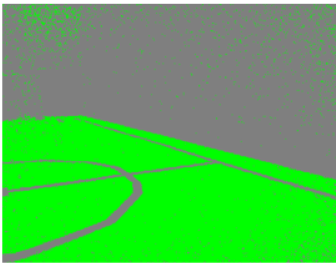
\includegraphics[width=0.4\textwidth]{pics/calGreen.PNG}
\caption{Exemplary configuration of the green color}
\label{fig:calGreen}
\end{figure}

\item Right-click into the ColorCalibration information view and press "save calibration".
\item Repeat this procedure for every color. One thing to metion is that the color of the ball is \textcolor{orange}{\textbf{orange}}, rather than \textcolor{red}{\textbf{red}}.
\item Finally, copy the new calibration to the robots by using the copyfiles-script:
\begin{lstlisting}
cd <BHuman-root-directory>/Make/Linux
./copyfiles <Develop/Debug/Release> <IP_AAA.BBB.CCC.DDD> -r
\end{lstlisting}
\end{enumerate}

\subsubsection{Camera Calibration}
There are three modes in Camera Calibration, namely automatic, default and manual. The following shows the process of automatic camera calibration.
\begin{enumerate}
\item Start the automatic camera calibration module:
\begin{lstlisting}
call CameraCalibrators/Automatic
\end{lstlisting}
\item Place the robot at a defined point on the field (e.g. Centerpoint (0,0)) and specify this spot in SimRobot with the following command: 
\begin{lstlisting}
set module:AutomaticCameraCalibrator:robotPose rotation= 0deg; translation = {x= 0; y=0;}
\end{lstlisting}
\item Start the calibration process:
\begin{lstlisting}
dr module:AutomaticCameraCalibrator:start
\end{lstlisting}
\item Start optimization process:
\begin{lstlisting}
dr module:AutomaticCameraCalibrator:optimize
\end{lstlisting}
\item Check if the created drawings of the field lines match the real field lines, if not, go back to point 3 and restart the calibration process.
\item Save the new calibration:
\begin{lstlisting}
save representation:CameraCalibration
\end{lstlisting}
\item Finally copy the new calibration to the robots by using the copyfiles-script:
\begin{lstlisting}
cd <BHuman-root-directory>/Make/Linux
./copyfiles <Develop/Debug/Release> <IP_AAA.BBB.CCC.DDD>
\end{lstlisting}
\end{enumerate}
However, it may finish the calibration with large deviation to the groundtruth. So the default and manual Calibration are recommended if there are large deviation. They can be implemented in the console in SimRobot by
\begin{lstlisting}
call CameraCalibrators/Default
\end{lstlisting}
Then the shortcut for different functions will shown in the console. The default calibration will calculate the result for the upper and lower camera according to the point chosen by us. The view of the camera can be changed by clicking on the screen and keep pressing \textit{shift}. But it seems that it is not very necessary to do it because usually this leads to the failure of convergence. What important for the point collection is that the point should be collected both in upper camera and in lower camera, so that it will converge faster and easier.  \\
If the Default Calibration is not satisfying, the manual calibration can be used with
\begin{lstlisting}
call CameraCalibrators/Manual
\end{lstlisting}
to finely tune the parameter. The direction of different axis can be known from trial and error. Figure~\ref{fig: CaCl} shows an example of the camera Calibration.
\begin{figure}[!htb]
    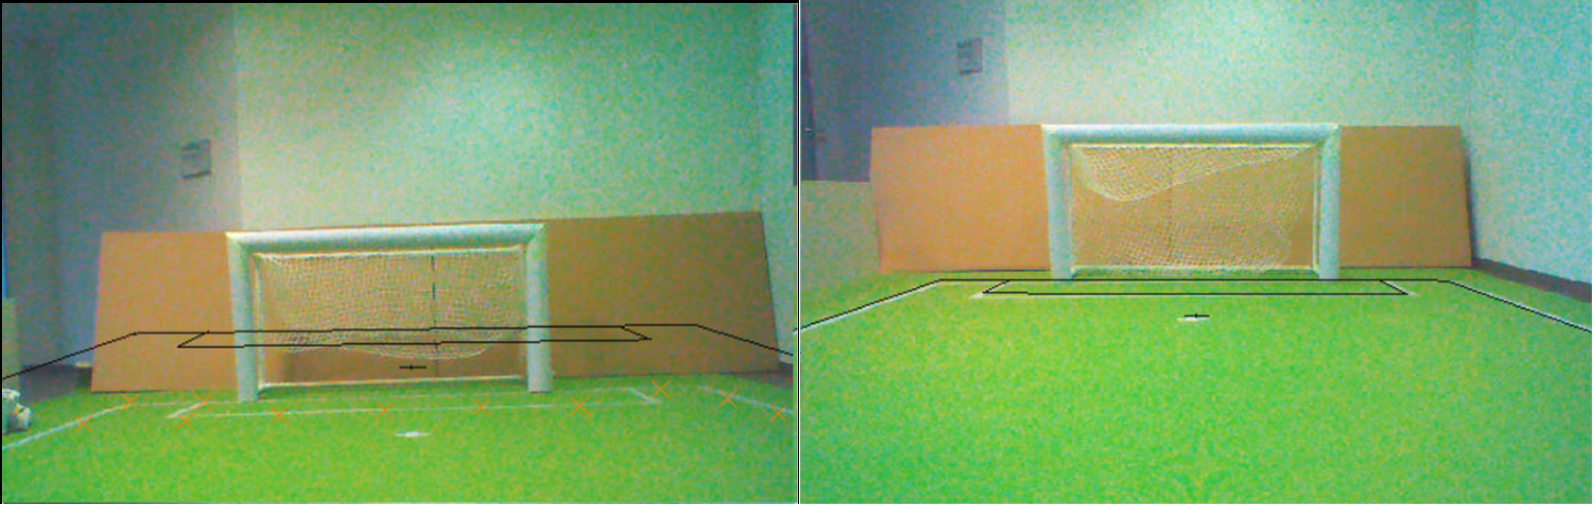
\includegraphics[width=\textwidth]{pics/Camera_Calibration}
    \centering
    \caption{Calibration: Before vs After}
    \label{fig: CaCl}
\end{figure}\\
\subsection{Playing a game}
After the previous steps, the robots should be able to play a real game in principle. \\
Do it and you will see many problems. \\
It's time to fix these problems by yourselves and start coding.\\
Some issues are opened in \emph{Gitlab} project page as mini-projects for the improvement. \\
(See \url{https://gitlab.lrz.de/ga35goz/RoboCup/issues})

\begin{thebibliography}{9}
\bibitem{BHuman2015}
  Thomas R{\"o}fer and Tim Laue and Jesse Richter-Klug and Maik Sch{\"u}nemann and Jonas Stiensmeier and Andreas Stolpmann and Alexander St{\"o}wing and Felix Thielke,
  \emph{{B}-{H}uman Team Report and Code Release 2015}.Only available online: \url{http://www.b-human.de/downloads/publications/2015/CodeRelease2015.pdf}
\end{thebibliography}
\end{document}